\begin{question}
\noindent A space research laboratory stores biological specimens in a cuboid-shaped sample container $ABCDEFGH$, as shown in the diagram.

\begin{center}
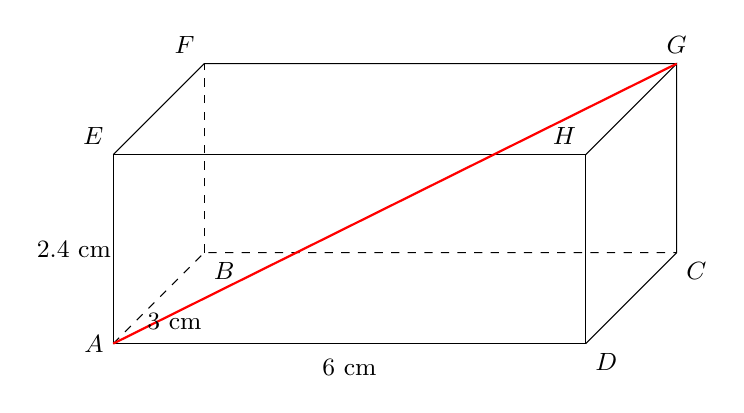
\begin{tikzpicture}[scale=1, transform shape]
    % Define the points of the cuboid
    \coordinate (A) at (0,0,0);
    \coordinate (B) at (0,0,-3);
    \coordinate (C) at (6,0,-3);
    \coordinate (D) at (6,0,0);
    \coordinate (E) at (0,2.4,0);
    \coordinate (F) at (0,2.4,-3);
    \coordinate (G) at (6,2.4,-3);
    \coordinate (H) at (6,2.4,0);

    % Draw the visible edges of the cuboid
    \draw (A) -- (D) -- (H) -- (E) -- cycle; % bottom face
    \draw (D) -- (C) -- (G) -- (H); % right face
    \draw (E) -- (F) -- (G); % top face

    % Draw the hidden edges of the cuboid
    \draw[dashed] (A) -- (B) -- (C);
    \draw[dashed] (B) -- (F);

    % Draw the diagonal from A to G
    \draw[thick, red] (A) -- (G);

    % Place the labels with smaller font size
    \node at (A) [left,font=\small] {$A$};
    \node at (B) [below right,font=\small] {$B$};
    \node at (C) [below right,font=\small] {$C$};
    \node at (D) [below right,font=\small] {$D$};
    \node at (E) [above left,font=\small] {$E$};
    \node at (F) [above left,font=\small] {$F$};
    \node at (G) [above,font=\small] {$G$};
    \node at (H) [above left, font=\small] {$H$};

    % Dimension labels
    \node at (3,-0.3,0) [font=\small] {$6$ cm};
    \node at (0.2,-0.3,-1.5) [font=\small] {$3$ cm};
    \node at (-0.5,1.2,0) [font=\small] {$2.4$ cm};
\end{tikzpicture}
\end{center}

\noindent The base $ABCD$ of the container is a rectangle with $AD = 6$ cm and $DC = 3$ cm.
The height of the container is $AE = 2.4$ cm.

\noindent Calculate the angle that the diagonal $AG$ makes with the base plane $ABCD$.
\vspace{5cm}
\begin{flushright}
\answerequnit{}{$^\circ$}{4}
\end{flushright}
\end{question}
